\section{Evaluation}\label{sec:experiments}
\subsection{Setup}
\subsubsection{Environment}
The experiments were performed on a single machine with two Intel Xeon Processor E5--2699 v4 CPUs, 64 GB of RAM,
and a 800GB SSD\@.
The machine has 22 cores and 44 threads.
Memory caches were dropped before each experiment to force disk loads.
\subsubsection{Datasets and Queries}
We use real-world data graphs~\cite{snapnets} listed in Table~\ref{tab:datasets}.
The datasets come from difference domains of application, and they range in different size.
The vertices and edges in the datasets are labeled randomly as in~\cite{DBLP:journals/pvldb/MhedhbiS19}.

The queries (Figure~\ref{img:queries}) are selected and edited from existing work~\cite{DBLP:conf/cloud/SerafiniMS17,DBLP:journals/pvldb/MhedhbiS19}.
The labels of vertices and edges are tagged randomly,
and they are represented by the color and the style of lines in Figure~\ref{img:queries}.
The queries we choose represent different topologies: trees, chains, and cyclic graphs.
$q_9$ --- $q_{12}$ are queries with multi-edges.
\begin{table}
  \caption{Datasets}\label{tab:datasets}
  \begin{tabular}{lrr}
    \toprule
    Name & $|V|$ & $|E|$ \\
    \midrule
    soc-Epinions (EP) & 76K & 509K \\
    web-Google (GO) & 876K & 5.1M \\
    web-BerkStan (BS) & 685K & 7.6M \\
    soc-LiveJournal (LJ) & 4.8M & 69M \\
    com-Orkut (OK) & 3.1M & 117.2M \\
    \bottomrule
  \end{tabular}
\end{table}

\begin{figure}[ht]
  \centering
  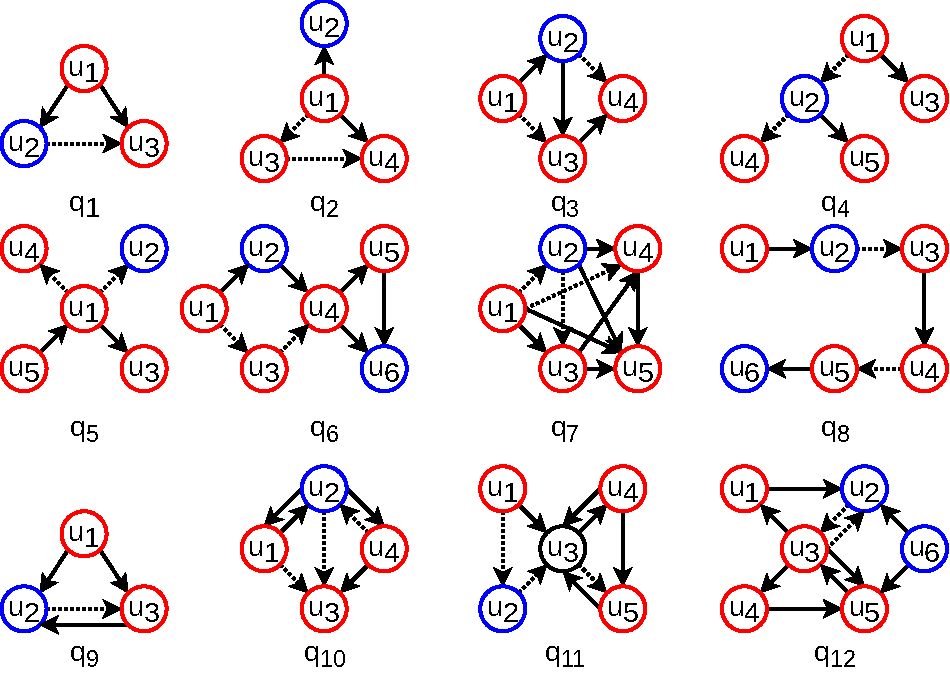
\includegraphics[width=0.5\textwidth]{img/queries.pdf}
  \caption{The queries.}\label{img:queries}
\end{figure}

\subsection{Preprocessing Cost}
We first study the preprocessing cost of SeqStar's vertex-centric storage engine.
The preprocessing incurs a external sort on the original graph data to generate the formatted data graph shown in Figure~\ref{img:data_graph}.
The cost is $\mathcal{O}(n \log n)$ where n is the size of the unsorted graph data.
We use 32-bit integers to store the vertex IDs, and 16-bit integers to store the vertex/edge labels.
As is shown in Figure~\ref{img:exp_preprocessing}, the preprocessing time grows linearly with respect to the size of graph data.
In fact, the preprocessing time of the vertex-centric storage is significantly smaller than the execution time of complex queries.

\begin{figure}[ht]
  \centering
  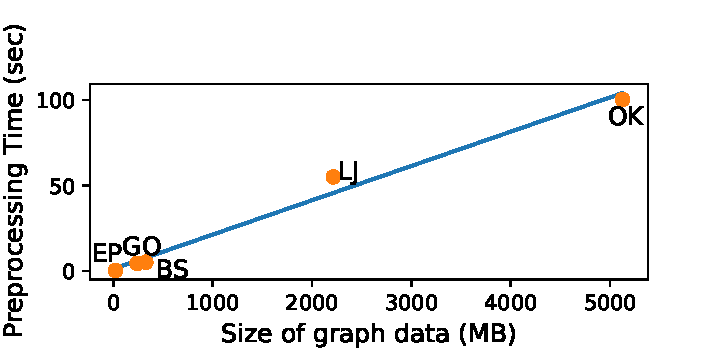
\includegraphics[width=0.4\textwidth]{img/exp_preprocessing.pdf}
  \caption{Preprocessing time of SeqStar.}\label{img:exp_preprocessing}
\end{figure}
\subsection{Comparative Performance}
We compare the overall performance of SeqStar against Graphflow~\cite{DBLP:journals/pvldb/MhedhbiS19} and Neo4j.

Graphflow is the state-of-the-art in-memory subgraph querying system,
and it is the fastest baseline we are aware of.
Graphflow is a JVM based system, and we set the maximum size of the JVM heap to 60GB to let it make full use of main memory.
However Graphflow does not support queries with multi-edges, i.e., $q_9$ --- $q_{12}$,
and it will report fake results for these queries\footnote{Graphflow will report matchings even the data does not contain multi-edges.}.
Therefore we use only $q_1$ --- $q_8$ to compare with Graphflow.
\begin{figure*}[ht]
  \centering
  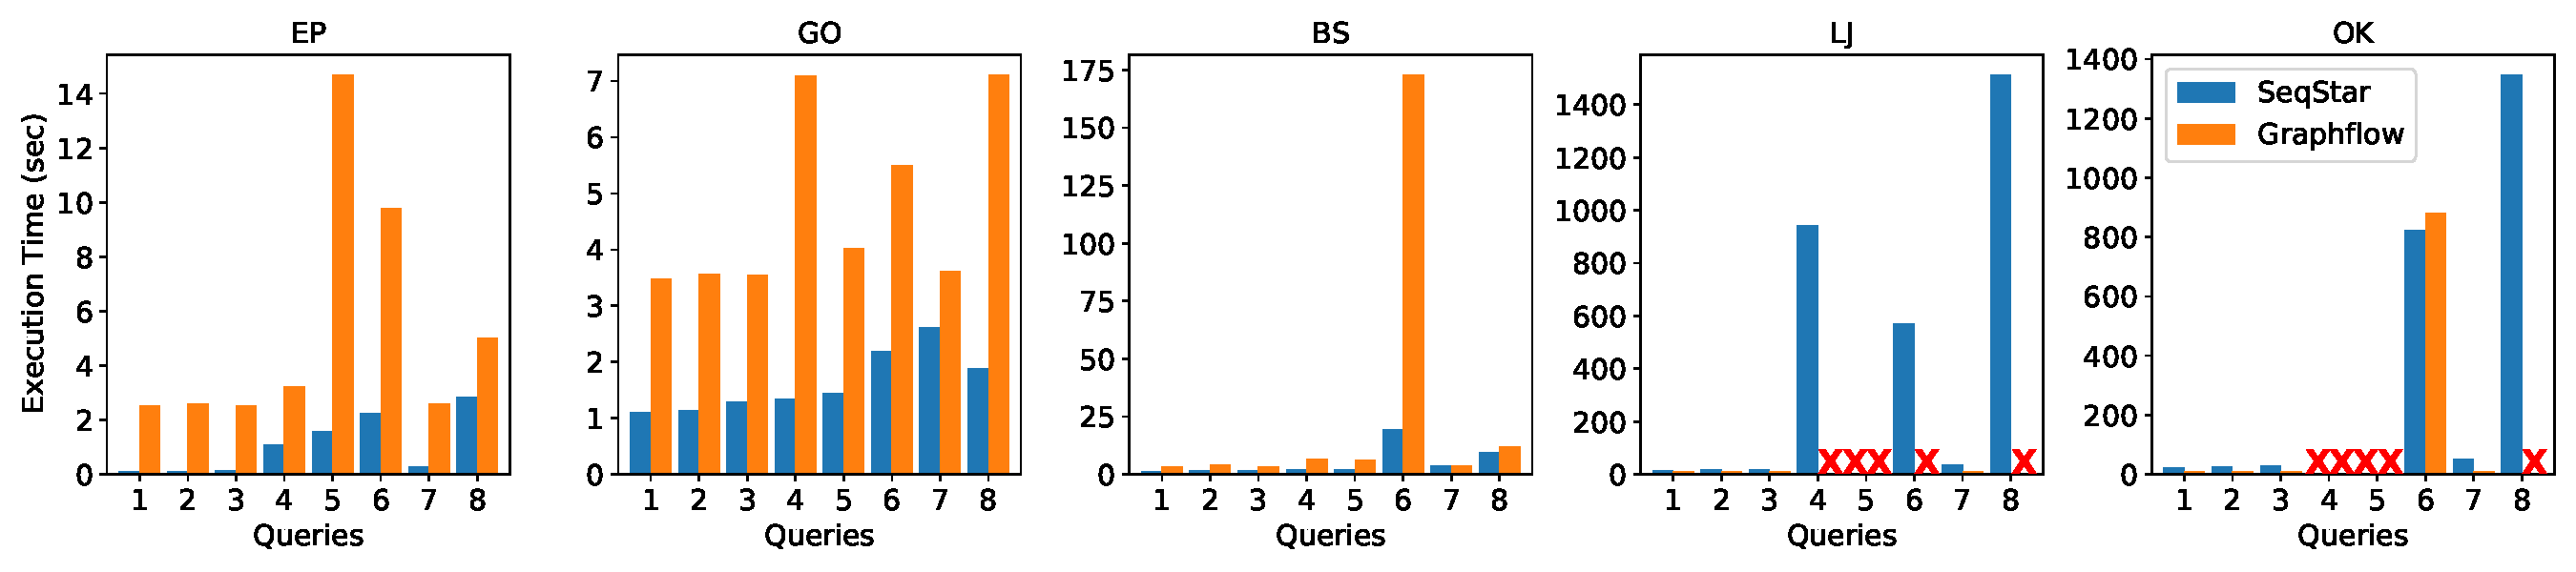
\includegraphics[width=\textwidth]{img/exp_compare.pdf}
  \caption{Execution time.}\label{img:exp_compare}
\end{figure*}

\subsection{Compression Ratio}
\subsection{Performance of Star Decompression}
\subsection{Parallelism of Pipeline Join}
